%!TEX root =  Report.tex
\chapter{Architectural Design}

\section{Architecture Diagram}
% Give block diagram showing the major components of your translator

\begin{figure}[h]
\begin{center}
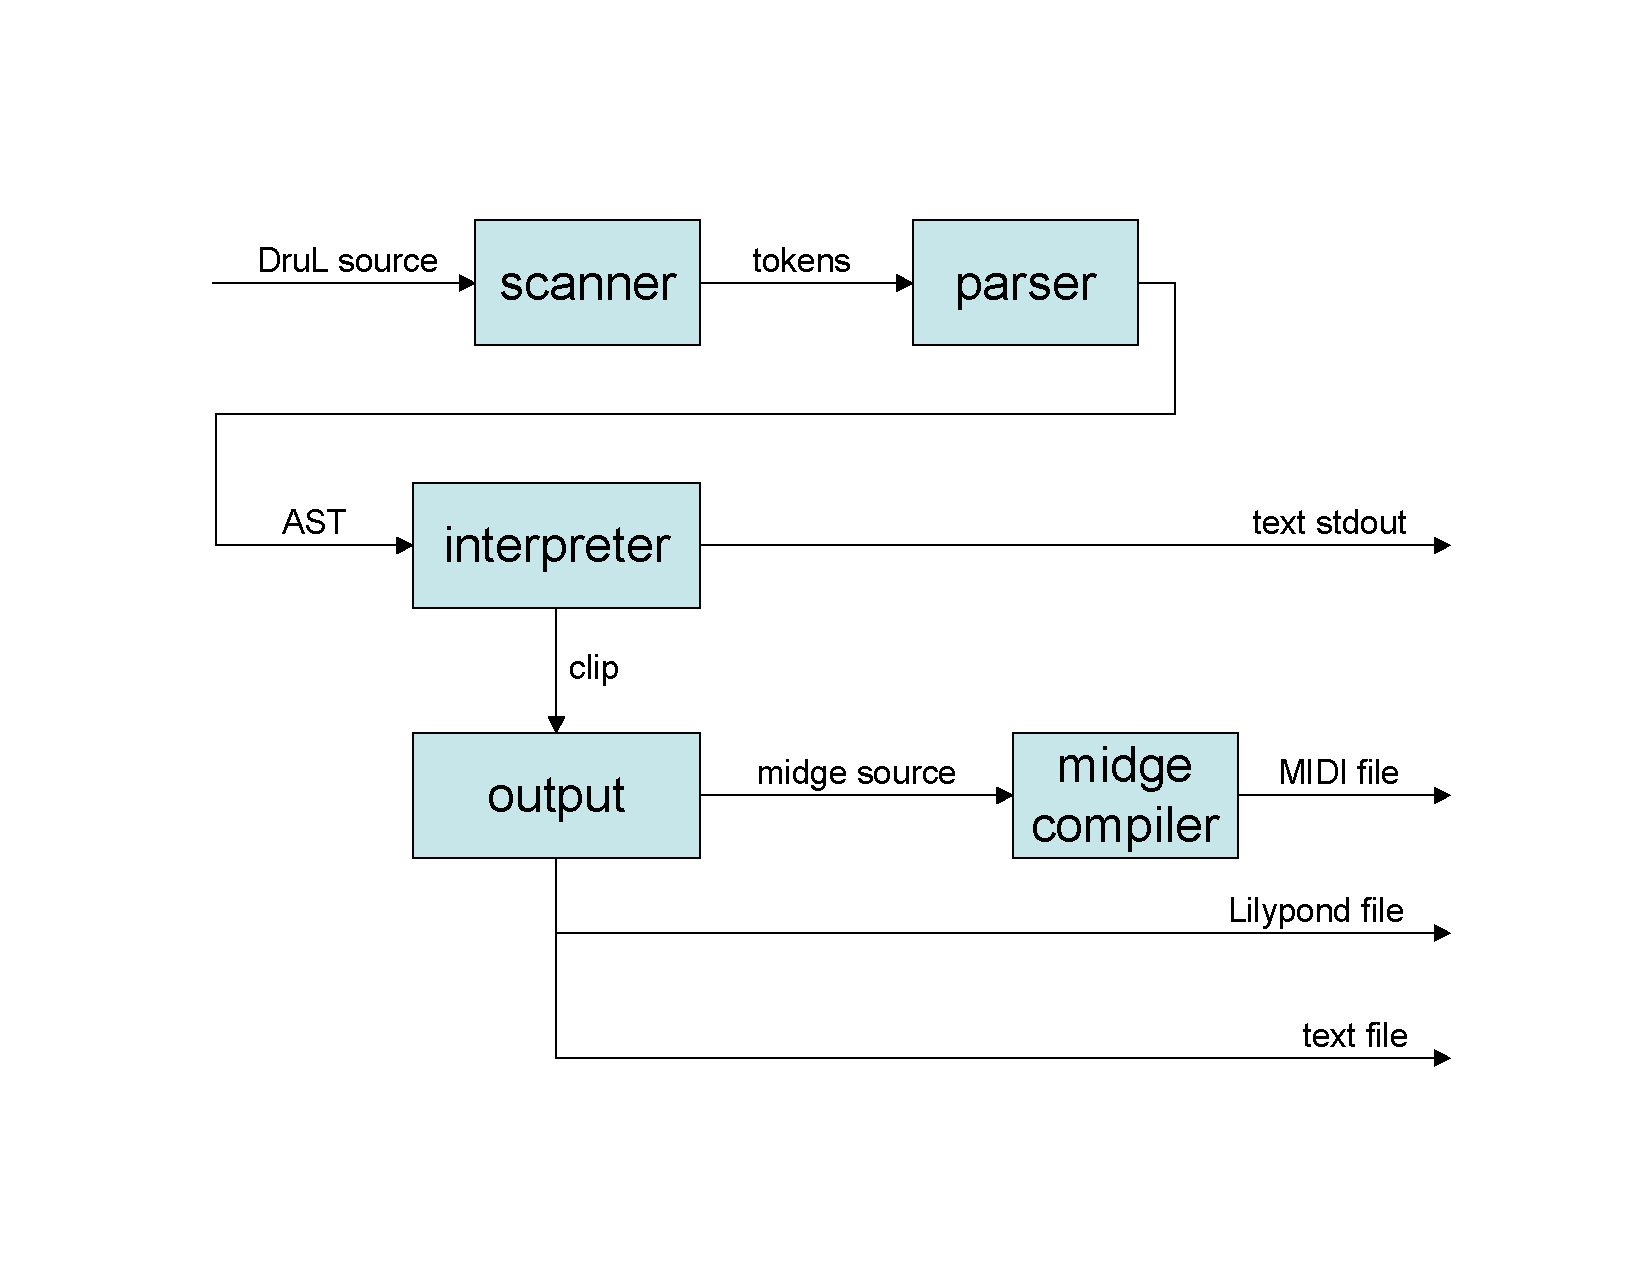
\includegraphics[width=.9\columnwidth]{Architecture_diagram.pdf}
\caption{Arrows heads on edges show direction of data-flow.}
%\label{fig:arch}}
\end{center}
\end{figure}

\section{Component Interfaces}

The DruL interpreter is (as shown above) architecturally very simple.  
\begin{enumerate}
\item The parser accepts a list of tokens from the scanner and builds a list of 
DruL statements (structured according to DruL's AST interface)  to pass to the main unit of the interpreter.  These components rely heavily on OCaml's Lexing and Parsing libraries.
\item
The interpreter is monolithic: with the exception of the output module, all of its major sub-components are built into one set of mutually recursive functions (in the file {\tt drul\_main.ml}--see appendix \ref{listing:main} on page \pageref{listing:main}).   This monolith takes the statement list produced by the parser, evaluates it step by step (performing semantic checks on each statement only when program flow arrives at it), and passes the resulting structures to the output library when appropriate.
\item
The output library is implemented as a set of simple utility functions: each 
takes a single DruL data structure and a small amount of extra data
(the exact breakdown is unfortunately not well standardized, and varies from output type to 
output type), and returns a string formatted for the appropriate output style.
\end{enumerate}

The monolithic design of the interpreter is necessitated by the single-pass approach taken to 
interpretation and by the dynamic typing of DruL variables: a re-implementation that included  compilation and checking passes
 could also maintain cleaner separation of concerns.

\section{Component Implemented By}
% State who implemented each component

\begin{tabular}{ | l | l | } \hline
	\textbf{File}        & \textbf{Author(s)} \\ \hline \hline
	drul\_scanner.mll    & Waseem             \\ \hline
	drul\_parser.mly     & all                \\ \hline
	drul\_ast.mli        & Ben and Rob        \\ \hline
	drul\_interpreter.ml & all                \\ \hline
	drul\_main.ml        & all                \\ \hline
	drul\_types.ml       & all                \\ \hline
	drul\_helpers.ml     & all                \\ \hline
	drul\_output.ml      & all                \\ \hline
\end{tabular}

